% --- PREÁMBULO ---
\documentclass[12pt, letterpaper]{article}

% --- PAQUETES ---
\usepackage[utf8]{inputenc}
\usepackage[spanish]{babel}
\usepackage{geometry}
\usepackage{graphicx}
\usepackage{placeins} 
\usepackage{url} % Para formatear URLs en la portada

% --- CONFIGURACIÓN DE MÁRGENES ---
\geometry{left=2.5cm, right=2.5cm, top=3cm, bottom=3cm}

% --- COMIENZO DEL DOCUMENTO ---
\begin{document}

% --- PORTADA PERSONALIZADA ---
\begin{titlepage}
    \centering

    % Encabezado de la universidad
    \textsc{\LARGE UNIVERSIDAD TECNOLÓGICA DE PEREIRA} \\[0.5cm]
    \textsc{\Large FACULTAD DE INGENIERÍAS} \\[0.5cm]
    \textsc{\large Programa de Ingeniería de Sistemas y Computación} \\[2cm]

    % Título del trabajo
    \rule{\textwidth}{0.4pt}\\[0.4cm]
    { \huge \bfseries Extensión para Visual Studio Code como simulador para procesador RISC-V \\[0.4cm] }
    \rule{\textwidth}{0.4pt}\\[2cm]

    % Información del estudiante
    \begin{flushleft}
    \textbf{Autor:} \\
    Amir Evelio Hurtado Mena \\
    \textbf{Código:} 1077997025 \\
    \textbf{Email:} \url{a.hurtado@utp.edu.co} \\[1cm]

    \textbf{Director:} \\
    (Nombre del Director) \\[2cm]
    \end{flushleft}

    % Información del proyecto
    \begin{center}
    \textbf{Área Temática:} Ingeniería de Software \\
    \textbf{Línea de Investigación:} Desarrollo de Software Aplicado \\[0.5cm]
    \textbf{Modalidad:} Proyecto de Aplicación \\[2cm]
    \end{center}

    \vfill % Empuja el contenido siguiente hacia el final de la página

    % Fecha
    Pereira, Colombia \\
    \today
\end{titlepage}


% --- TABLA DE CONTENIDOS ---
\newpage
\tableofcontents


% --- INTRODUCCIÓN ---
\newpage 
\section{Introducción}
La Arquitectura de Computadores es una materia fundamental en la carrera de Ingeniería de Sistemas y Computación, ya que permite entender cómo funciona el hardware que ejecuta todo el software que creamos. Sin embargo, los conceptos sobre el funcionamiento interno de un procesador, como los registros, las unidades de control y los ciclos de instrucción, suelen ser muy abstractos y dificiles de asimilar para los estudiantes que cursan la asignatura en la Universidad Tecnológica de Pereira.

Esta dificultad a menudo genera un obstáculo en el proceso de aprendizaje, ralentizando el avance de las clases y dejando vacíos conceptuales en los futuros profesionales. Para abordar este problema, este proyecto propone el desarrollo de una herramienta de software: una extensión para el editor de código Visual Studio Code que funciona como un simulador gráfico e interactivo de un procesador con arquitectura RISC-V, tanto en su versión monociclo como segmentada.

El objetivo es ofrecer a estudiantes y docentes un recurso que traduzca las operaciones complejas del procesador en visualizaciones claras y fáciles de seguir. De esta manera, se busca fortalecer la comprensión de los temas clave de la materia, haciendo el aprendizaje más práctico, intuitivo y efectivo, y mejorando así la calidad de la formación de los ingenieros de la universidad.


% --- PLANTEAMIENTO DEL PROBLEMA ---
\section{Planteamiento del problema}

\subsection{Antecedentes (Contextualización del problema)}
La enseñanza de la Arquitectura de Computadores presenta desafios pedagógicos bien documentados en la literatura académica. Uno de los principales retos identificados es la dificultad para conectar la teoría con la práctica (Bridging Theory and Practice). Los estudiantes a menudo luchan por trasladar el conocimiento teórico a una aplicación tangible, lo que dificulta la comprensión de cómo se ejecutan los programas a nivel de sistema. Para abordar esto, varios autores proponen el uso de sistemas interactivos y laboratorios de aprendizaje asistido por computador (CAL) que permiten a los estudiantes visualizar la ejecución de programas e inspeccionar los detalles de implementación hasta el nivel de transferencia de registros (\cite{djordjevic2008}, \cite{oztekin2011}).

Otro desafio clave es la comprensión conceptual (Conceptual Understanding) de sistemas que son complejos e intangibles. Investigaciones señalan que muchos estudiantes, incluso de ciencias de la computación, tienen ideas erróneas fundamentales sobre cómo funcionan realmente los programas, un problema que requiere atención desde el diseño del currículo (\cite{senske2014}). En este contexto, el uso de herramientas de visualización de la ejecución se ha propuesto como una solución efectiva para ayudar a los estudiantes a comprender estos sistemas (\cite{oztekin2011}).

Por lo tanto, la literatura académica no solo confirma la existencia de estas barreras de aprendizaje, sino que también respalda el desarrollo de herramientas interactivas y visuales, como la propuesta en este proyecto, como un camino viable para mejorar significativamente la experiencia educativa en esta área fundamental.

\subsection{Causas (qué está causando el problema)}
La causa principal del problema en la asignatura de Arquitectura de Computadores de la UTP es la brecha existente entre la teoría abstracta enseñada en clase y la falta de herramientas prácticas que permitan a los estudiantes visualizar y experimentar con dichos conceptos. Esta situación fue validada a través de una encuesta realizada a 57 estudiantes del programa que ya habían cursado la materia. Los resultados revelan la magnitud del desafío: un contundente 86\% de los estudiantes calificó el proceso de comprensión de la arquitectura de un computador y su implementación en hardware como "Complejo" o "Muy complejo", lo que demuestra que no se trata de una percepción aislada, sino de una dificultad generalizada en el alumnado (Ver Gráfico \ref{fig:grafico1}).

\begin{figure}[h!]
    \centering
    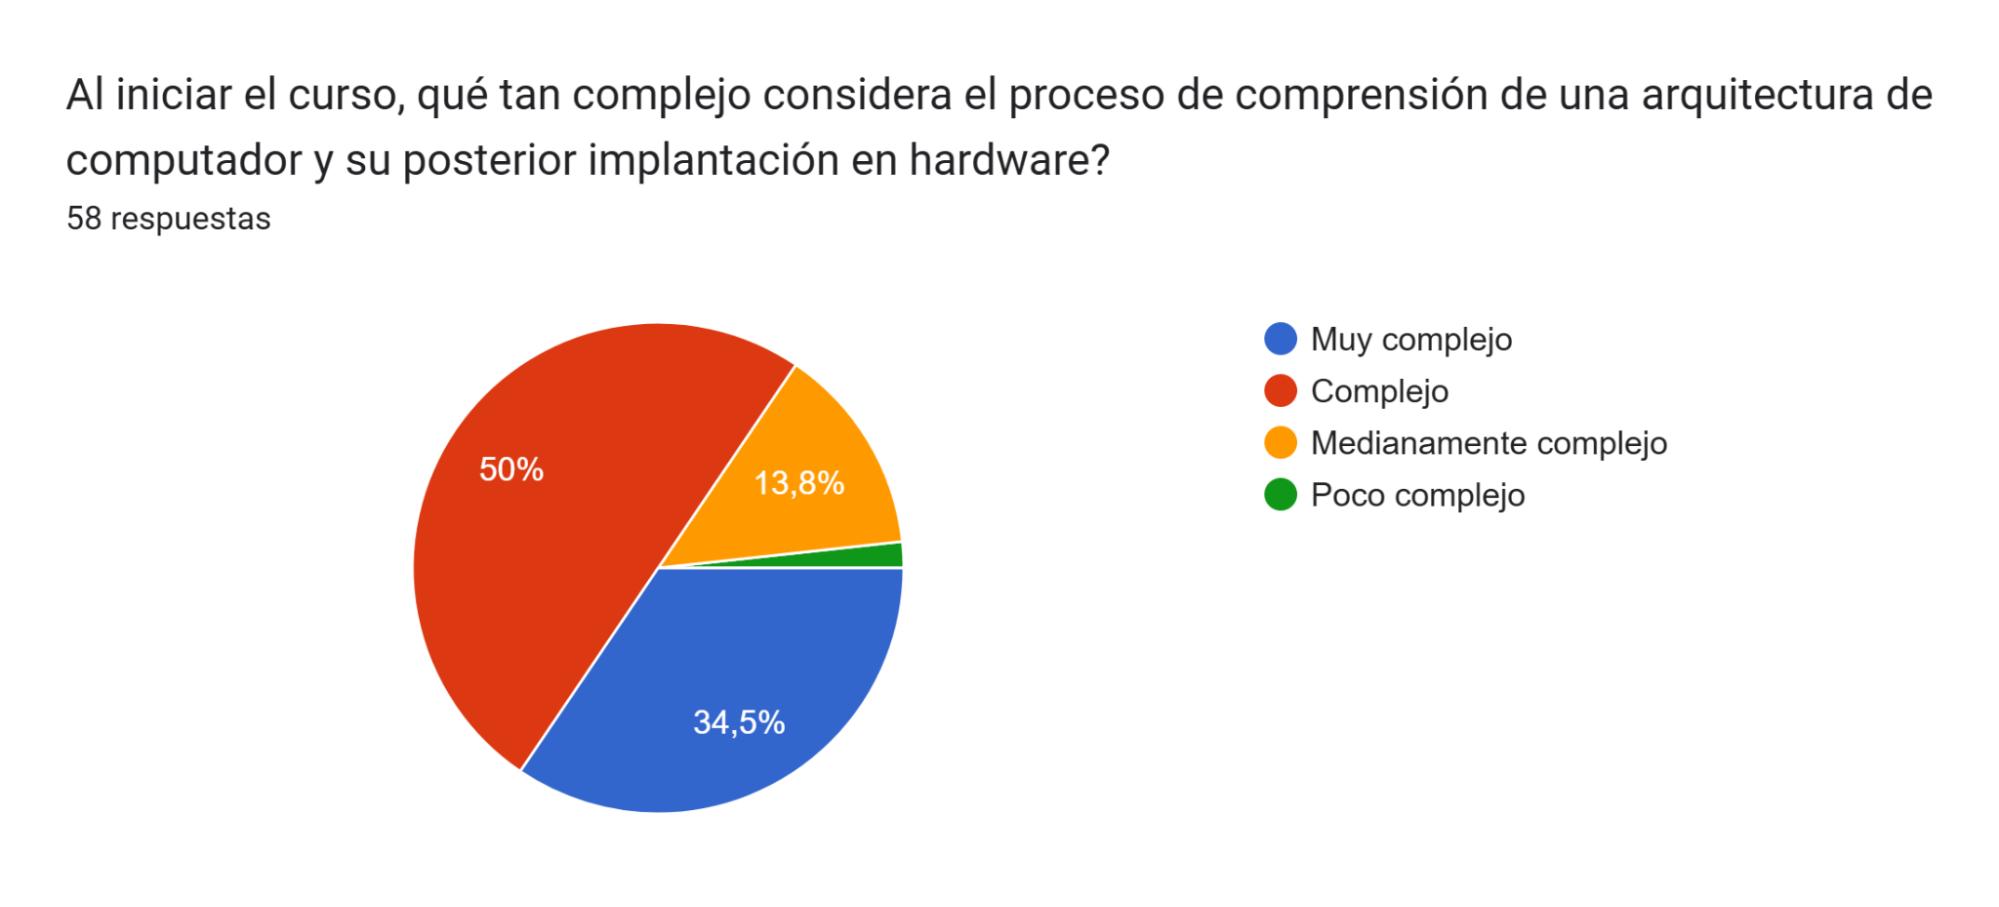
\includegraphics[width=0.7\textwidth]{figura1.png}
    \caption{Resultados sobre la complejidad percibida.}
    \label{fig:grafico1}
\end{figure}

Más importante aún, la encuesta también indagó sobre la solución a esta dificultad. Al preguntarles sobre la necesidad de una nueva herramienta, la respuesta fue abrumadora: un 91.1\% de los estudiantes (sumando las categorías "Muy necesario" y "Necesario") afirmó que la inclusión de una herramienta tecnológica para visualizar los conceptos sería clave para un mejor aprendizaje (Ver Gráfico \ref{fig:grafico2}). Estos datos demuestran que la causa del problema no es una falta de interés por parte del alumnado, sino una necesidad directa y explícita de un recurso didáctico interactivo que les permita conectar los conceptos abstractos con una representación visual y práctica. La herramienta propuesta en este proyecto busca, por lo tanto, atacar directamente esta causa raíz.

\begin{figure}[h!]
    \centering
    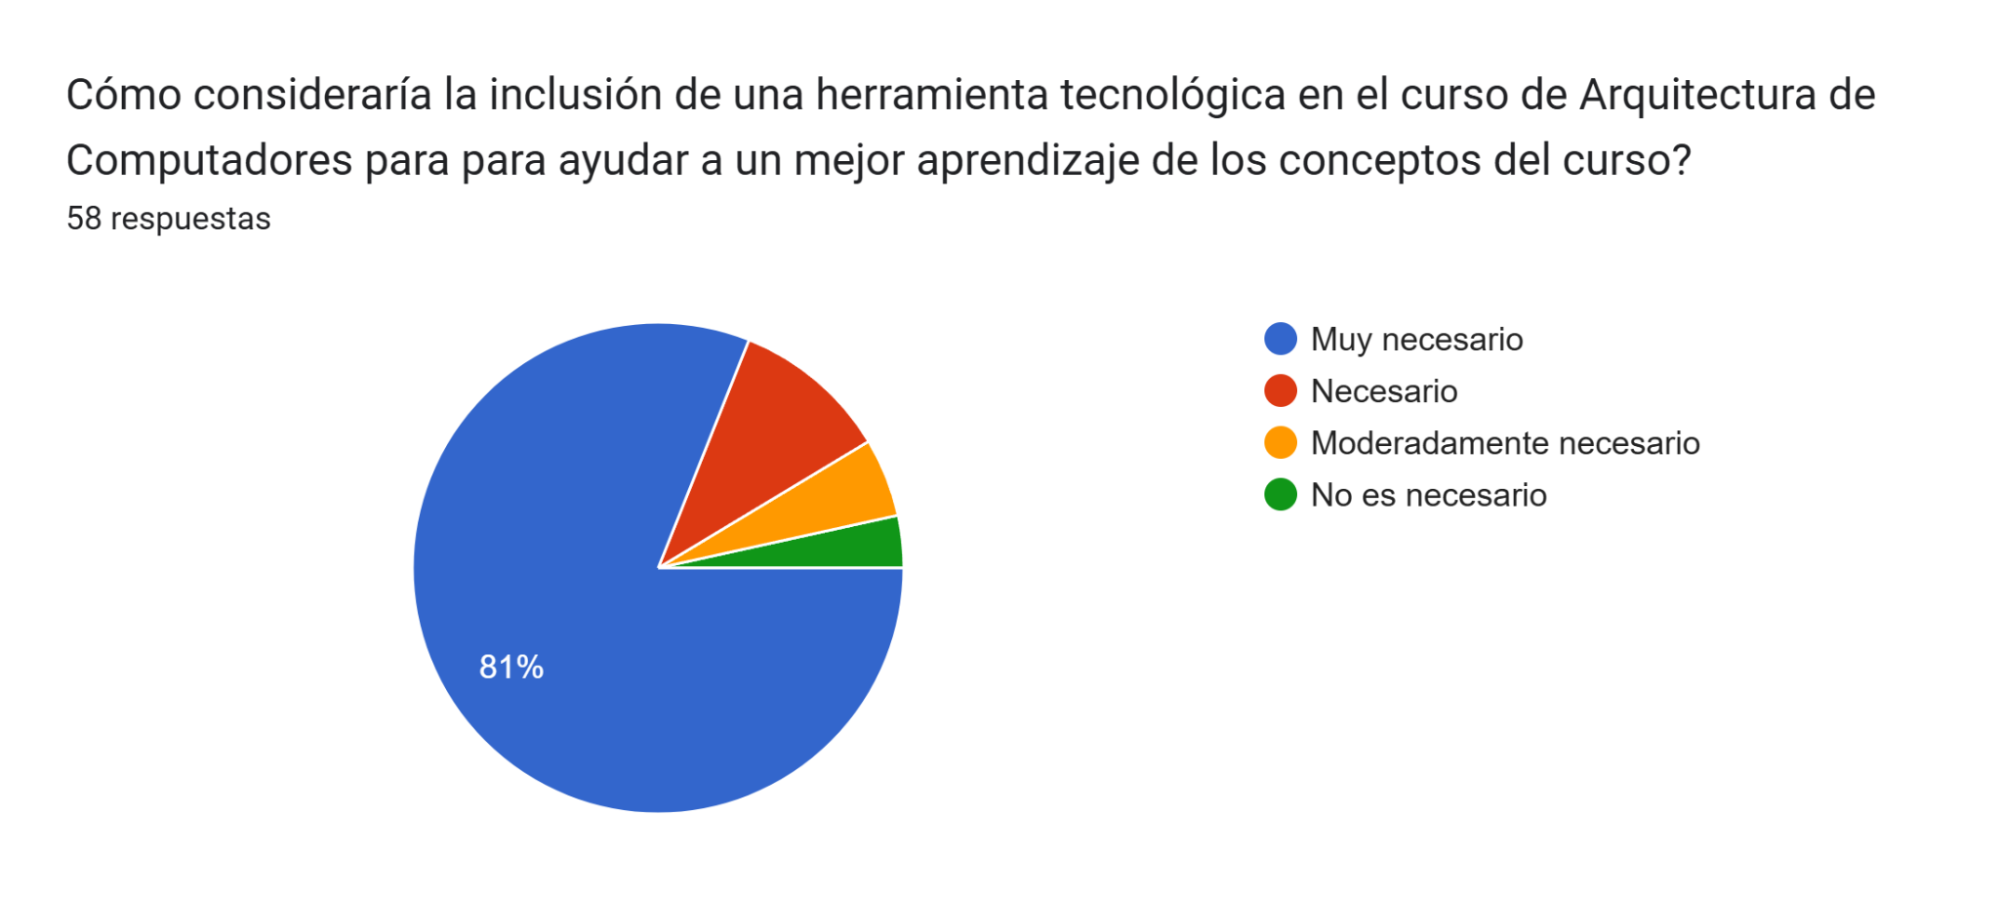
\includegraphics[width=0.8\textwidth]{figura2.png}
    \caption{Necesidad de una herramienta tecnológica según los estudiantes.}
    \label{fig:grafico2}
\end{figure}

% --- BARRERA PARA LAS IMÁGENES ANTES DE LA SIGUIENTE SECCIÓN ---
\FloatBarrier 

\subsection{Definición del problema}
Los estudiantes de la asignatura de Arquitectura de Computadores del programa de Ingeniería de Sistemas y Computación de la UTP presentan dificultades significativas para comprender los procesos internos de un procesador (monociclo y segmentado).

\subsection{Consecuencias (de no resolver el problema)}
De no abordarse este problema, las consecuencias afectan a múltiples niveles. Para los estudiantes, implica una base conceptual débil que puede perjudicar su desempeño en materias posteriores que dependen de estos conocimientos, además de generar frustración y desinterés por el área del hardware. Para los docentes, significa tener que invertir más tiempo en reforzar conceptos básicos, ralentizando el avance del temario y limitando la posibilidad de profundizar en temas más avanzados. A largo plazo, para el programa académico, esto representa un riesgo en la calidad de la formación, ya que sus egresados podrían tener vacíos en un área fundamental de la ingeniería de sistemas, lo que podría impactar negativamente su perfil profesional en el mercado laboral.


% --- JUSTIFICACIÓN ---
\section{Justificación}
La realización de este proyecto se justifica plenamente por su alto impacto en el proceso formativo de los estudiantes de Ingeniería de Sistemas y Computación de la UTP, así como por los aportes que ofrece tanto a los docentes como al programa académico. A continuación, se detallan los beneficios desde distintas perspectivas:

\subsection{Justificación Pedagógica y Académica}
Este proyecto ataca directamente una barrera de aprendizaje validada. Como lo demostró la encuesta, el 86\% de los estudiantes considera complejo el proceso de comprensión de la materia, y un 91.1\% reclama una herramienta tecnológica para facilitar este proceso. Por lo tanto, el principal beneficio es para el estudiante, quien contará con un recurso interactivo diseñado para:
\begin{itemize}
    \item Transformar lo abstracto en tangible: Permitirá visualizar el flujo de datos, el estado de los registros y la ejecución de instrucciones paso a paso, haciendo que los conceptos teóricos cobren vida.
    \item Fomentar el aprendizaje autónomo: Los estudiantes podrán experimentar y probar código a su propio ritmo, reforzando los conocimientos vistos en clase y resolviendo dudas de forma práctica.
    \item Aumentar la motivación y reducir la frustración: Al facilitar la comprensión, se espera un mayor interés por una de las áreas más fundamentales y áridas de la carrera.
\end{itemize}
Para los docentes, la herramienta se convertirá en un valioso recurso que les permitirá explicar temas complejos de manera más eficiente y gráfica, optimizando el tiempo en el aula y asegurando un nivel de comprensión más homogéneo en el grupo.

\subsection{Justificación Tecnológica}
Desde el punto de vista tecnológico, el proyecto es relevante por el desarrollo de una solución de software específica y moderna. La creación de una extensión para Visual Studio Code, uno de los editores de código más utilizados en el mundo profesional, asegura que la herramienta se integre de forma natural en el entorno de trabajo de los estudiantes. Además, el enfoque en la arquitectura RISC-V, un estándar abierto y en pleno auge, garantiza que el conocimiento adquirido a través del simulador sea actual y pertinente para el futuro de la industria del hardware.

\subsection{Justificación Institucional}
Para el programa de Ingeniería de Sistemas y Computación de la UTP, este proyecto representa una oportunidad para fortalecer sus métodos de enseñanza. La implementación de esta herramienta demuestra un compromiso con la mejora continua de la calidad educativa y con la atención a las necesidades de sus estudiantes. En resumen, este trabajo no solo resuelve un problema académico concreto y medido, sino que también aporta una solución tecnológica moderna y fortalece el ecosistema de aprendizaje del programa, generando un beneficio claro para toda la comunidad universitaria involucrada.


% --- OBJETIVOS ---
\section{Objetivos}

\subsection{Objetivo General}
Desarrollar una extensión de software para Visual Studio Code que simule de forma gráfica y textual el funcionamiento de un procesador RISC-V con arquitecturas monociclo y segmentada, para facilitar la comprensión de los conceptos fundamentales de la asignatura Arquitectura de Computadores.

\subsection{Objetivos específicos}
\begin{enumerate}
    \item Elaborar el documento de especificación de requisitos funcionales y no funcionales del simulador, detallando las características de visualización necesarias para las arquitecturas RISC-V monociclo y segmentada. \textbf{Entregable:} Documento de Especificación de Requisitos.
    \item Diseñar la arquitectura de software de la extensión para Visual Studio Code y los prototipos de la interfaz de usuario (mockups), garantizando que la interacción sea intuitiva y responda a los requisitos definidos. \textbf{Entregable:} Documentos de diseño de arquitectura y prototipos/mockups de la interfaz.
    \item Construir los módulos funcionales del simulador según el diseño establecido, implementando la carga de código, la ejecución paso a paso y la visualización en tiempo real de los componentes del procesador. \textbf{Entregable:} Código fuente de la extensión (versión funcional).
    \item Ejecutar un plan de pruebas funcionales para verificar el correcto funcionamiento del simulador y realizar pruebas piloto con un grupo de usuarios (estudiantes y docentes) para evaluar la usabilidad y pertinencia pedagógica de la herramienta. \textbf{Entregable:} Informe de resultados de pruebas funcionales y de las pruebas piloto.
\end{enumerate}



% --- METODOLOGÍA ---
\section{Metodología}

\subsection{Marco Metodológico}
Para el desarrollo de este proyecto de aplicación, se empleará una Metodología de Desarrollo de Software Basada en Prototipos. Esta metodología es ideal para proyectos donde la interfaz de usuario y la experiencia de interacción son críticas para el éxito, como es el caso de esta herramienta educativa. El enfoque se centra en construir versiones funcionales tempranas (prototipos) que pueden ser evaluadas por los usuarios finales (estudiantes y docentes) para validar y refinar los requisitos desde el inicio del proceso, evitando así errores y malentendidos en fases posteriores del desarrollo (\cite{yang2019}).

El proceso se dividirá en cuatro fases principales, que se alinean directamente con los objetivos específicos del proyecto:

\subsubsection{Fase 1: Definición y Especificación}
En esta etapa inicial, se realizará el levantamiento y la documentación de los requisitos. Las actividades incluyen:
\begin{itemize}
    \item \textbf{Estudio conceptual:} Se analizarán los temas clave de las arquitecturas RISC-V monociclo y segmentada que presentan mayor dificultad, basándose en la bibliografia de la asignatura y los resultados de la encuesta inicial.
    \item \textbf{Documentación:} Se elaborará el documento de especificación de requisitos, detallando las funcionalidades (ej. carga de código, ejecución paso a paso) y los requisitos no funcionales (ej. rendimiento, diseño responsivo).
\end{itemize}

\subsubsection{Fase 2: Diseño y Prototipado}
Con los requisitos claros, se procederá a diseñar la solución.
\begin{itemize}
    \item \textbf{Diseño de Arquitectura:} Se definirá la estructura interna de la extensión, los componentes de software y cómo se comunicarán entre sí.
    \item \textbf{Diseño de Interfaz (UI/UX):} Se crearán los prototipos visuales y de interacción (mockups) de la herramienta utilizando software de diseño como Figma. Estos prototipos se centrarán en intentar tener una experiencia intuitiva.
\end{itemize}

\subsubsection{Fase 3: Construcción e Implementación}
Esta es la fase de codificación.
\begin{itemize}
    \item \textbf{Configuración del entorno:} Se preparará el ambiente de desarrollo para extensiones de Visual Studio Code.
    \item \textbf{Desarrollo incremental:} Se construirán las funcionalidades del simulador de forma modular, empezando por el núcleo (la simulación del procesador) y luego la capa de visualización.
\end{itemize}

\subsubsection{Fase 4: Validación y Evaluación}
En esta última fase se verificará que la herramienta cumple con lo esperado.
\begin{itemize}
    \item \textbf{Descripción de la unidad de muestreo:} La "unidad de muestreo" serán los participantes de las pruebas piloto. Se seleccionará un grupo de estudiantes que estén cursando, y al menos un docente del área.
    \item \textbf{Descripción del "tratamiento" y su aplicación:} El "tratamiento" será el uso guiado de la extensión de Visual Studio Code. A los participantes se les entregarán ejercicios prácticos y se les pedirá que utilicen el simulador para resolverlos.
    \item \textbf{Información a registrar:} Se recolectará información cualitativa y cuantitativa a través de observación directa, encuestas de satisfacción y reporte de errores.
    \item \textbf{Análisis de la información:} Los resultados de las pruebas se analizarán para identificar puntos de mejora en la herramienta y para redactar el informe final que valida el cumplimiento del proyecto.
\end{itemize}

\subsection{Actividades}
A continuación, se desglosan las actividades principales derivadas de cada objetivo específico:
\begin{itemize}
    \item \textbf{Objetivo 1: Elaborar el documento de especificación de requisitos...}
    \begin{itemize}
        \item Actividad 1.1: Investigar y sintetizar los conceptos de RISC-V monociclo y segmentado más relevantes para la simulación.
        \item Actividad 1.2: Redactar la primera versión del documento de requisitos funcionales y no funcionales.
        \item Actividad 1.3: Validar el documento de requisitos con el director del proyecto.
    \end{itemize}
    \item \textbf{Objetivo 2: Diseñar la arquitectura de software...}
    \begin{itemize}
        \item Actividad 2.1: Crear el diagrama de la arquitectura de la extensión.
        \item Actividad 2.2: Diseñar los mockups y el flujo de usuario de la interfaz gráfica.
        \item Actividad 2.3: Documentar las decisiones de diseño.
    \end{itemize}
    \item \textbf{Objetivo 3: Construir los módulos funcionales...}
    \begin{itemize}
        \item Actividad 3.1: Desarrollar el motor de simulación para la arquitectura monociclo.
        \item Actividad 3.2: Desarrollar el motor de simulación para la arquitectura segmentada.
        \item Actividad 3.3: Implementar la interfaz gráfica y su conexión con el motor de simulación.
    \end{itemize}
    \item \textbf{Objetivo 4: Ejecutar un plan de pruebas funcionales...}
    \begin{itemize}
        \item Actividad 4.1: Elaborar el plan de pruebas y los casos de uso para la prueba piloto.
        \item Actividad 4.2: Seleccionar y convocar a los participantes para la prueba.
        \item Actividad 4.3: Ejecutar las sesiones de la prueba piloto.
        \item Actividad 4.4: Recolectar y analizar los resultados de las pruebas.
        \item Actividad 4.5: Redactar el informe final de validación.
    \end{itemize}
\end{itemize}


% --- APORTES DEL PROYECTO ---
\section{Aportes del Proyecto}
\begin{itemize}
    \item \textbf{Software Funcional:} El principal aporte es la extensión para Visual Studio Code, una herramienta de software completamente funcional para la simulación gráfica e interactiva de un procesador RISC-V en sus arquitecturas monociclo y segmentada. Este software quedará a disposición del programa de Ingeniería de Sistemas y Computación para su uso libre en la asignatura de Arquitectura de Computadores.
    \item \textbf{Documentación Técnica del Proyecto:} Se entregarán todos los documentos que respaldan el proceso de ingeniería de software realizado, los cuales incluyen: el Documento de Especificación de Requisitos, los Documentos de Diseño y el Informe de Pruebas y Validación.
    \item \textbf{Manual de Usuario:} Se elaborará un documento guía que explique de manera clara y sencilla cómo instalar, configurar y utilizar la extensión de software, dirigido tanto a estudiantes como a docentes.
\end{itemize}


% --- MARCO REFERENCIAL ---
\section{Marco Referencial}

\subsection{Marco Teórico}
En este capítulo se definen los conceptos técnicos fundamentales que sustentan el desarrollo del proyecto. Se explican las tecnologías y arquitecturas clave necesarias para comprender tanto el problema abordado como la solución propuesta.

\subsubsection{Arquitectura RISC-V}
RISC-V es una arquitectura de conjunto de instrucciones (ISA) basada en los principios de un computador con un conjunto reducido de instrucciones (RISC). A diferencia de otras arquitecturas comerciales, RISC-V es completamente gratuita y de código abierto, lo que permite una amplia adopción y personalización (\cite{poojary2025}). Su diseño es inherentemente modular, lo que significa que consiste en un conjunto base de instrucciones simples al que se le pueden añadir extensiones para funcionalidades específicas. Esta flexibilidad la hace ideal para una gran variedad de aplicaciones, desde pequeños sistemas embebidos hasta computadores de alto rendimiento (\cite{mallidu2023}).

\subsubsection{Procesador Segmentado (Pipelined)}
Esta arquitectura mejora drásticamente el rendimiento al dividir la ejecución de una instrucción en múltiples etapas más cortas que operan en paralelo, de forma similar a una línea de ensamblaje. El modelo clásico para RISC-V se divide en cinco etapas: 1. Búsqueda (Fetch), 2. Decodificación (Decode), 3. Ejecución (Execute), 4. Memoria (Memory) y 5. Escritura (Write Back) (\cite{khairullah2022}). Al permitir que varias instrucciones se procesen simultáneamente en diferentes etapas, se logra un rendimiento mucho mayor que en el diseño monociclo. No obstante, esta paralelismo introduce complejidades como los "riesgos" (hazards), que deben ser gestionados para asegurar el correcto funcionamiento (\cite{ihtemam2024}).

\subsection{Estado del Arte}
A continuación, se revisan otras herramientas de software que existen para enseñar arquitectura de computadores. Esto ayuda a entender por qué este proyecto es diferente y necesario. Herramientas como MARS (MIPS Assembler and Runtime Simulator), que es muy usada para enseñar la arquitectura MIPS, tienen una interfaz llena de información que puede confundir a un principiante (\cite{vollmar2007}). Igualmente, programas más nuevos para RISC-V como VRV o la página web WebRISC-V, son muy potentes, pero para usarlos bien, el estudiante ya necesita entender qué significa cada cosa que ve en la pantalla (\cite{giorgi2019}, \cite{krim2025}).


% --- BIBLIOGRAFÍA ---
\newpage
\bibliographystyle{plain}
\bibliography{referencias} % Le dice a LaTeX que use el archivo "referencias.bib" (sin la extensión)


\end{document}